\section{Introduction}
As our society is becoming increasingly dependent on technology, the demand for better and more efficient technologies is growing. One kind of technology which has been really important since its conception during the second world war by Alan Turing is computers \cite{Nielsen:2010}. The field of computer science has been researched a lot during the second half of the 20th century but has hit a fundamental problem. Our current classical computers have reached a limit where the transistors cannot get any smaller without quantum mechanics causing issues \cite{Nielsen:2010}. This has prompted research into quantum technologies such as quantum computers and quantum simulations \cite{Nielsen:2010}. 

To properly understand how quantum mechanical systems work, it is important to understand what happens to them when they are interacted with, during for example a measurement \cite{Jordan:2024}. It is also this interaction with a quantum system, which has prompted many interpretations of quantum mechanics and given rise to what is known as the measurement problem \cite{Jordan:2024}. The measurement problem is a fundamental philosophical problem in quantum mechanics, which arises since a quantum mechanical state evolves deterministically according to the Schrödinger equation, but collapses probabilistically when measured or interacted with \cite{Jordan:2024}.

It is also interesting to see how such a system can be manipulated to create a certain state which can be used for a specific purpose. This could include, but is not limited to, creating a qubit state to be used in a quantum computer or a state which can simulate a certain physical system \cite{Nielsen:2010}. Here it is important to understand the effect feedback has on a measured system, and how to utilize this to create a desired state \cite{Annby-Andersson:2024}.

To create technologies based on quantum mechanical phenomena, we need systems where the quantum mechanical properties dominate. One way to achieve this is to cool the system to very low temperatures. There are several ways to do this, some common ways include laser cooling, evaporative cooling and cavity cooling \cite{De-Sousa:2025}. This thesis however, will focus on measurement and feedback based cooling, where the system is continuously measured, and the result is fed to a feedback loop that affects the system in a way that decreases the energy. 

\begin{figure}
    \centering
    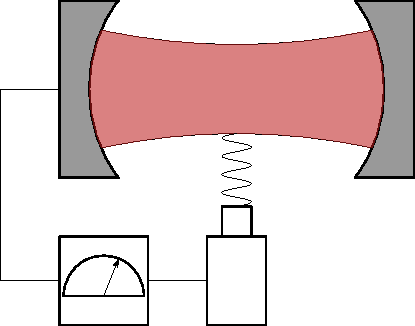
\includegraphics[]{figures/systemFirstVersion.pdf}
    \caption{The system and feedback apparatus considered in this thesis.}
    \label{fig:system}
\end{figure}

The abstract system considered in the thesis can be seen in Fig. \ref{fig:system}. There are however, numerous physical realizations. It could be mechanical motion of a particle confined in a harmonic potential, for example an electron confined in a potential generated by lasers. It could also be realized as an optical or microwave cavity where photons are oscillating. Superconducting circuits are also a good example of a physical realization.

This thesis will look at a quantum harmonic oscillator which is coupled to an environment. Thus creating an open quantum system whose state is temperature dependent. The system will be measured continuously using weak measurements with a feedback loop to control the system. The goal is to see how the system evolves under these conditions, and how the feedback loop can be changed and manipulated to observe different behaviours.

\subsection{Outline}
The remaining is organized as follows: Section 2 starts by introducing the theoretical framework central to this thesis by first defining what we mean by a quantum harmonic oscillator as well as shortly introducing the density matrix formalism of quantum mechanics. Then, we move on to discuss open quantum systems and the mathematical framework for the evolution of this type of system, and here we define a Markovian master equation in Lindblad form. We then move on to discussing measurements on open systems as well as feedback control, in the same mathematical formalism. In section 3, we use what has been discussed to derive equations of motion for the QHO as well as then computing the energy of the system. These results also allow analysing the stability of the system both with and without feedback. In section 4, there is a discussion of the relevancy of the results obtained in section 3, as well as mentions of a few applications.


